\section{Examples \textbf{Needed: redo these once decision is made on normalized/unnormalized SAX. Also want more examples}}
\subsection{Surgical procedure}
In this analysis, clusters were defined based on surgical procedure category. Icons are shown in Figure \ref{fig:surgerytype_beta2} corresponding to $\beta=2$, Figure \ref{fig:surgerytype_beta5} to $\beta=5$, and Figure \ref{fig:surgerytype_beta10} to $\beta=10$.

\begin{figure}[h]
  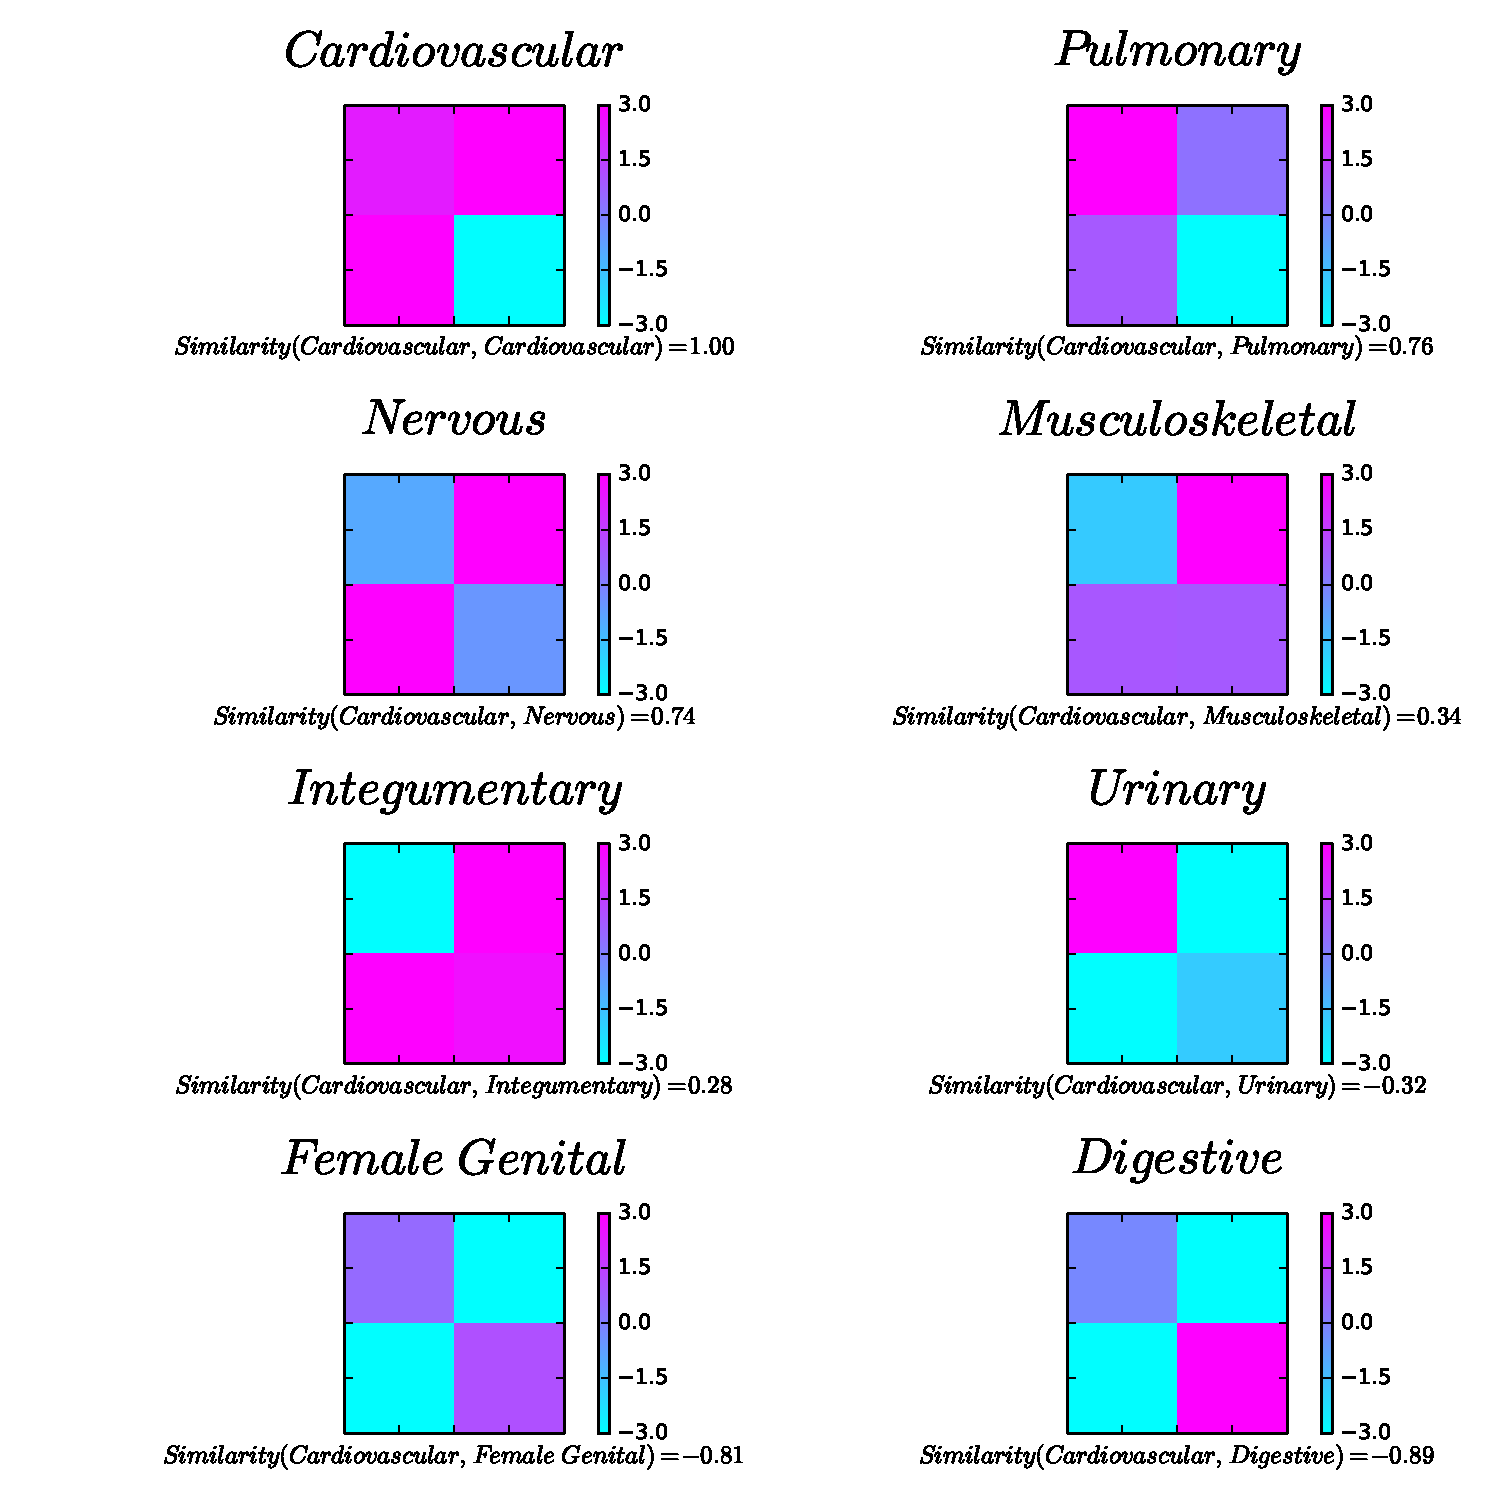
\includegraphics[scale=0.4]{./Figures/surgerytype_beta2.pdf}\\
  \caption{Icons for clusters of patients based on type of surgical procedure, $\beta=2$. Icons are sorted in descending similarity from the cluster of patients who underwent cardiovascular surgery.}\label{fig:surgerytype_beta2}
\end{figure}

\begin{figure}[h]
  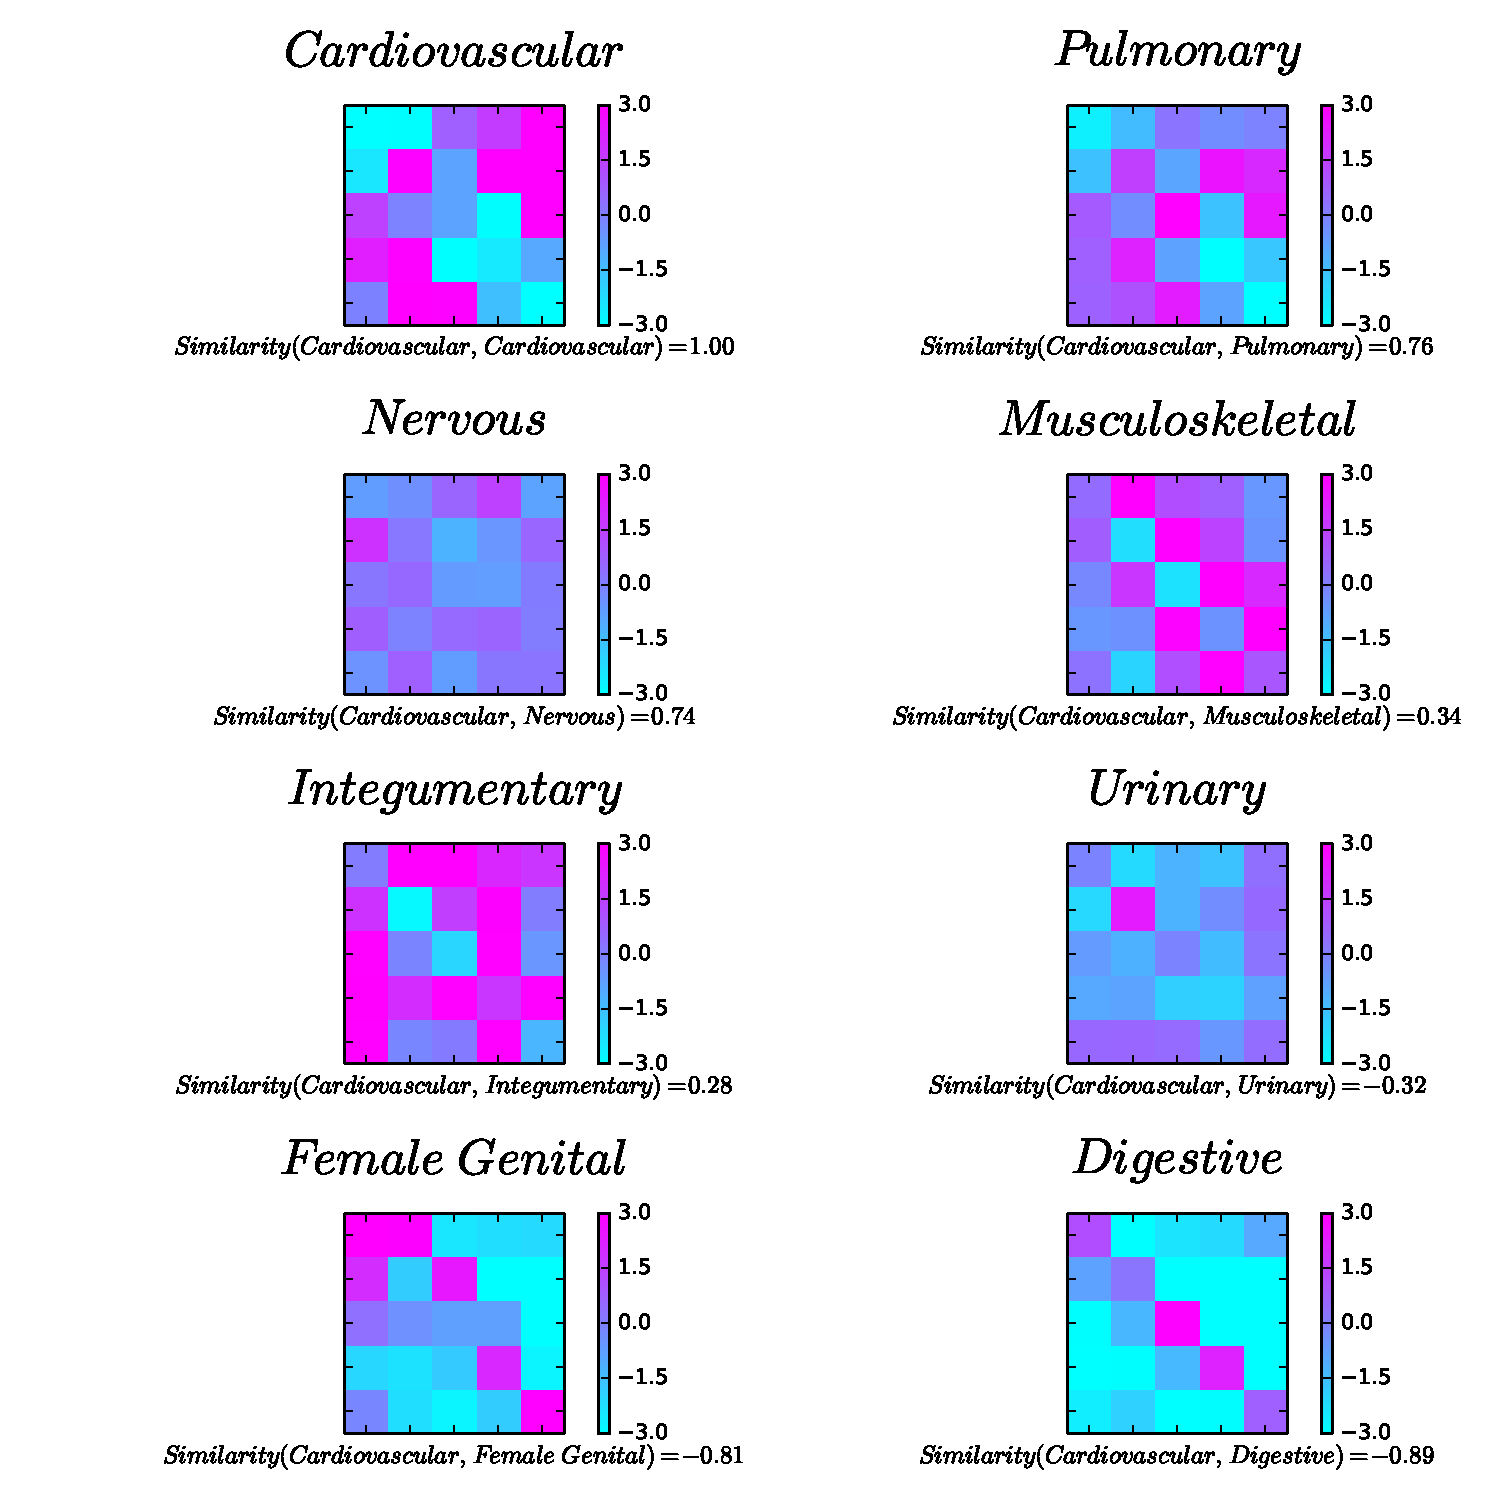
\includegraphics[scale=0.4]{./Figures/surgerytype_beta5.pdf}\\
  \caption{Icons for clusters of patients based on type of surgical procedure, $\beta=5$. Icons are sorted in descending similarity from the cluster of patients who underwent cardiovascular surgery.}\label{fig:surgerytype_beta5}
\end{figure}

\begin{figure}[h]
  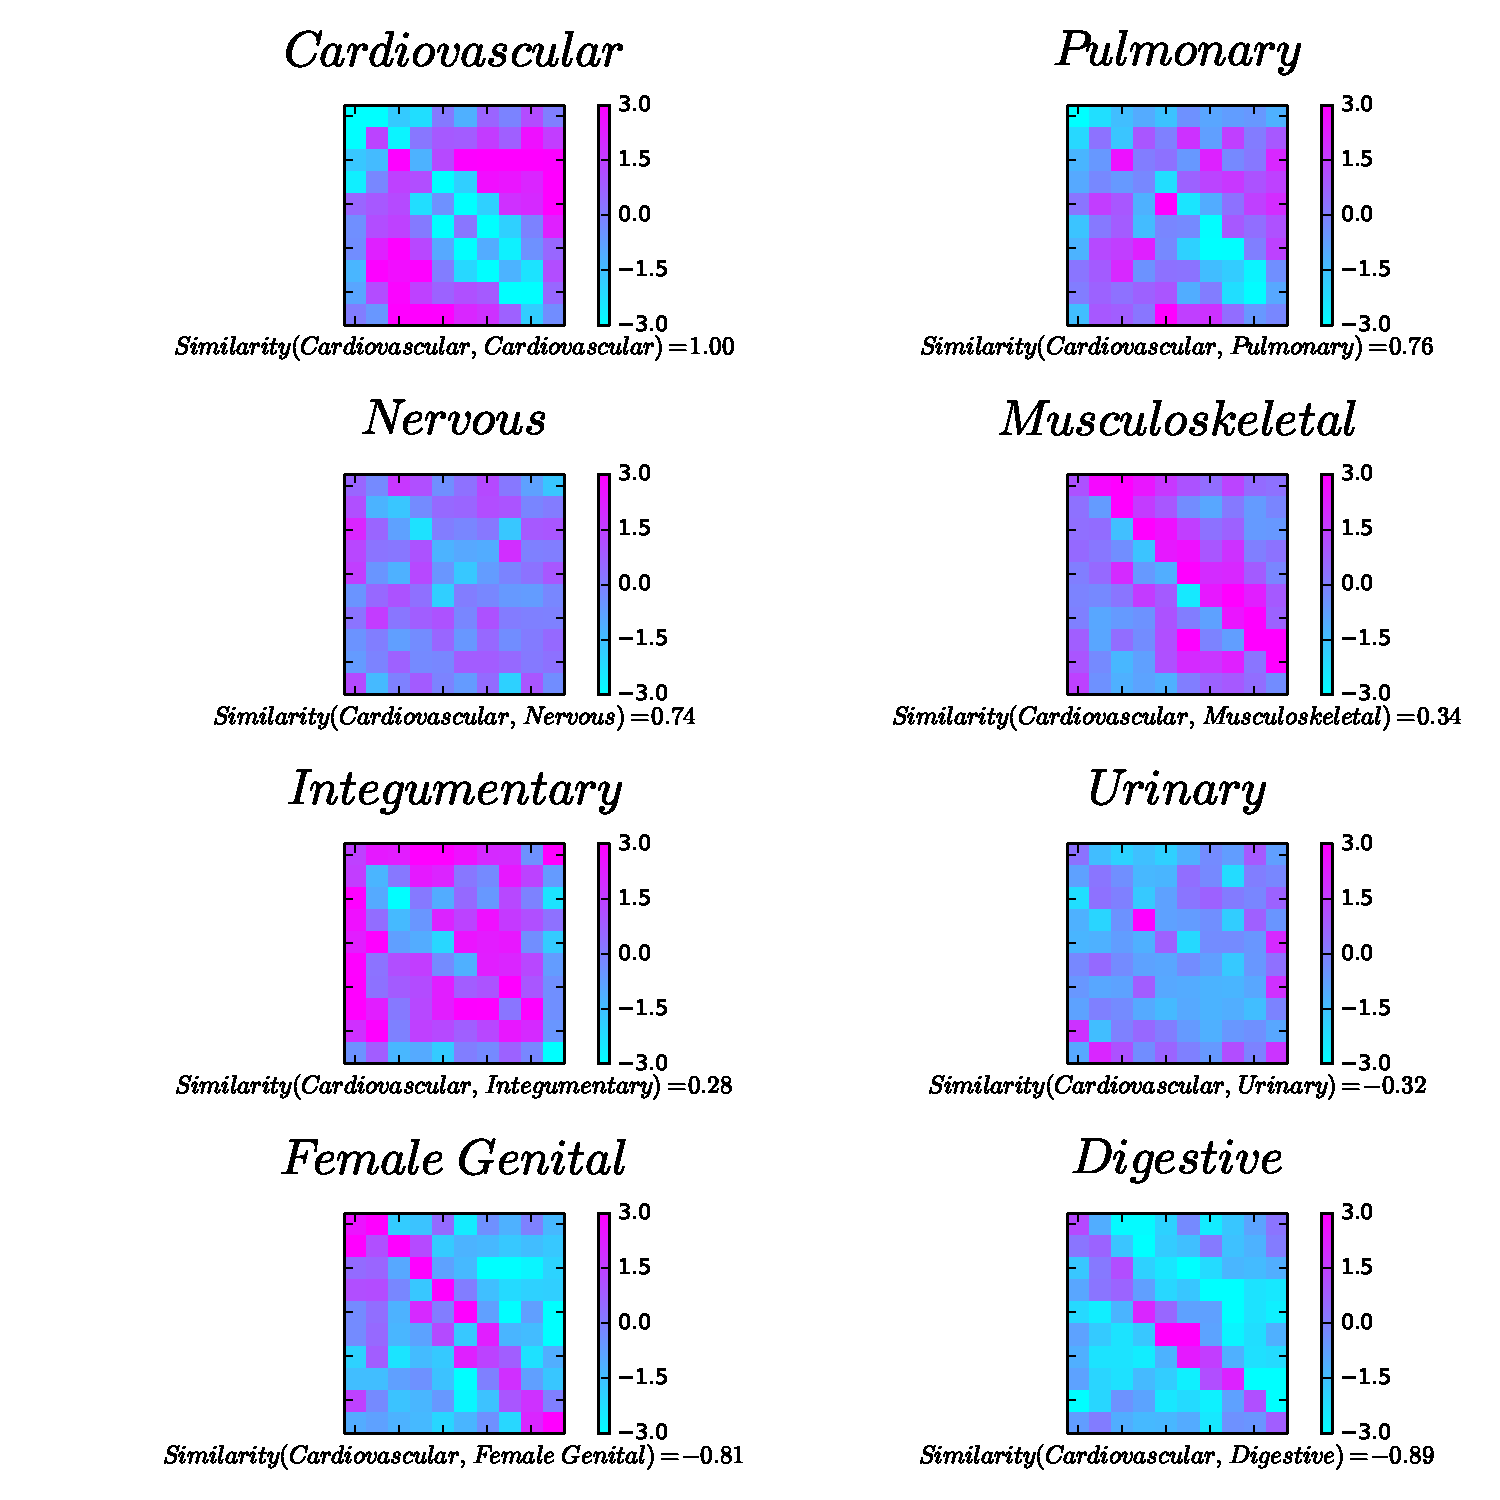
\includegraphics[scale=0.4]{./Figures/surgerytype_beta10.pdf}\\
  \caption{Icons for clusters of patients based on type of surgical procedure, $\beta=10$. Icons are sorted in descending similarity from the cluster of patients who underwent cardiovascular surgery.}\label{fig:surgerytype_beta10}
\end{figure}
